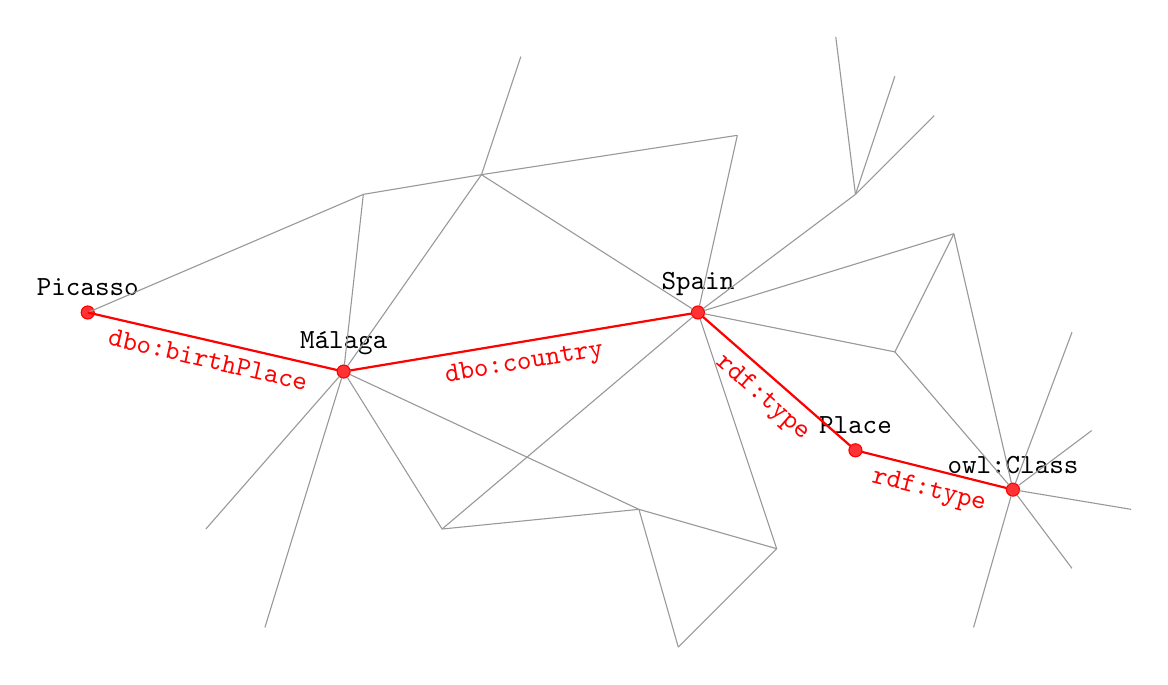
\begin{tikzpicture}
[   cnode/.style={draw=black,fill=#1,minimum width=3mm,circle},
    rnode/.style={draw=black,fill=#1,minimum width=6mm, minimum height=5mm, rectangle},
    rel/.style={draw=gray!80},
    edge/.style={draw=red, thick, red},
    vertex/.style={draw=red, fill=red!80, scale=0.5, circle}
]
\node (0) at (-2.25, 2.75) {};
\node[vertex, label={\texttt{Málaga}}] (1) at (-4, 0.25) {};
\node[vertex, label={\texttt{Spain}}] (2) at (0.5, 1) {};
\node (3) at (3.75, 2) {};
\node[vertex, label={\texttt{Place}}] (4) at (2.5, -0.75) {};
\node (5) at (1, 3.25) {};
\node (6) at (-0.25, -1.5) {};
\node[vertex, label={\texttt{owl:Class}}] (7) at (4.5, -1.25) {};
\node (8) at (5.25, 0.75) {};
% Extra nodes
\node (9) at (-2.75, -1.75) {};
\node (10) at (-5, -3) {};
\node (11) at (-5.75, -1.75) {};
\node[vertex, label={\texttt{Picasso}}] (12) at (-7.25, 1) {};
\node (13) at (-3.75, 2.5) {};
\node (14) at (2.25, 4.5) {};
\node (15) at (-1.75, 4.25) {};
\node (16) at (2.5, 2.5) {};
\node (17) at (1.5, -2) {};
\node (18) at (0.25, -3.25) {};
\node (19) at (4, -3) {};
\node (20) at (6, -1.5) {};
\node (21) at (3, 0.5) {};
\node (22) at (5.5, -0.5) {};
\node (23) at (5.25, -2.25) {};
\node (24) at (3.25, -2) {};
\node (25) at (-0.75, -2.75) {};
\node (26) at (3, 4) {};
\node (27) at (3.5, 3.5) {};

\draw [style=rel] (1) to  (0.center);
\draw [style=edge] (1) to node[below, sloped] {\texttt{dbo:country}} (2);
\draw [style=rel] (0.center) to (2);
\draw [style=rel] (0.center) to (5.center);
\draw [style=rel] (5.center) to (2);
\draw [style=rel] (1) to (6.center);
\draw [style=edge] (2) to node[below, sloped] {\texttt{rdf:type}} (4);
\draw [style=edge] (4) to node[below, sloped] {\texttt{rdf:type}} (7);
\draw [style=rel] (8.center) to (7);
\draw [style=rel] (3.center) to (7);
\draw [style=rel] (2) to (3.center);
% EXTRA EDGES
\draw [style=rel] (15.center) to (0.center);
\draw [style=rel] (0.center) to (13.center);
\draw [style=rel] (13.center) to (1);
\draw [style=rel] (12.center) to (13.center);
\draw [style=edge] (12.center) to node[below, sloped] {\texttt{dbo:birthPlace}} (1);
\draw [style=rel] (11.center) to (1);
\draw [style=rel] (10.center) to (1);
\draw [style=rel] (9.center) to (1);
\draw [style=rel] (9.center) to (6.center);
\draw [style=rel] (6.center) to (18.center);
\draw [style=rel] (18.center) to (17.center);
\draw [style=rel] (6.center) to (17.center);
\draw [style=rel] (17.center) to (2);
\draw [style=rel] (2) to (16.center);
\draw [style=rel] (16.center) to (14.center);
\draw [style=rel] (3.center) to (21.center);
\draw [style=rel] (2) to (21.center);
\draw [style=rel] (21.center) to (7);
\draw [style=rel] (7) to (19.center);
\draw [style=rel] (7) to (20.center);
\draw [style=rel] (16.center) to (26.center);
\draw [style=rel] (16.center) to (27.center);
\draw [style=rel] (7) to (23.center);
\draw [style=rel] (7) to (22.center);
\draw [style=rel] (9.center) to (2);

\end{tikzpicture}